\documentclass{article}
\usepackage{setspace}

% Language setting
% Replace `english' with e.g. `spanish' to change the document language
\usepackage[english]{babel}
% For Code
\usepackage{listings}

% Set page size and margins
% Replace `letterpaper' with `a4paper' for UK/EU standard size
\usepackage[letterpaper,top=2cm,bottom=2cm,left=3cm,right=3cm,marginparwidth=1.75cm]{geometry}

% Useful packages
\usepackage{amsmath}
\usepackage{graphicx}
\usepackage[colorlinks=true, allcolors=blue]{hyperref}
\onehalfspacing

\title{262 Final Project: Distributed Federated Learning}
\author{Neeraj Chandra & Ben Altschuler}

\begin{document}
\maketitle


\section{Introduction}

For our final project we built a distributed federated learning platform that can scale to $n$ nodes within the same network. Each node is able to contribute their own data to the global model. The source code for this project can be found at: \url{https://github.com/soccernee/decentralized_federated_learning}.
  

\subsection{Federated Learning}
Federated Learning (FL) is a machine learning approach that allows multiple devices to collaboratively learn a shared prediction model while keeping the training data decentralized. In FL, each device trains a local model using its own data and then sends only the updated model parameters to a central server or leader. The leader then aggregates the parameters from all the devices to update the global model, which is then sent back to the nodes for further training or inference. This approach enables collaborative learning while maintaining data privacy and reducing the need for data transfer to a central location.

\subsection{Motivation}
Use cases of federated learning include Health outcome predictions from the data on IoT devices and Hospitals, loan default predictions from bank data, and data locality compliance. As federated learning grows in popularity and use casses, there should be a decentralized method of training and distributing the model to ensure that data security is maintained. In this paper we present a decentralized federated learning platform.    

\section{Implementation}

\subsection{Leader}

To orchestrate our network of $n$ nodes we implemented a client-server architecture with one leader at any time. The leader maintains a set of the \nameref{sec:an} and the most up-to-date \nameref{sec:mw}. The leader sends model updates and the most up-to-date set of all active nodes in the network to the client nodes through a \nameref{sec:hb}.  The function of the leader can be assumed by any node in the system if the current leader crashes. The new leader is chosen through \nameref{sec:le}.


\subsubsection{Active Nodes}
\label{sec:an}
The leader maintains two vital pieces of information: the set of active nodes and the most up-to-date model weights. The set of active nodes is used by the server to know who should be sent a heartbeat. The set of actives nodes is used by the nodes when the leader goes down. At this moment they must speak to each other to figure out who the new leader should be. The set of active nodes is maintained within a class so that the same set can be accessed by the main function and the threads containing the gRPC server. The set of active nodes is kept as a dictionary because it allows the program to identify nodes that have been deregistered without decreasing the size of the active\_nodes dictionary. This ensures we do not run into issues where a thread loops through an object that decreases in size resulting in an thread Exception. Below is selection of the ActiveNodes class.

\begin{lstlisting}[language=Python]
    class ActiveNodes():
        def __init__(self):
            self.active_nodes = {}
            self.recent_additions = []
            self.recent_deletions = []
            ...
        
        def add_node(self, node_id, node):
            self.active_nodes[node_id] = node
            self.recent_additions.append(node_id)
            ...

        def remove_node(self, node_id):
            self.active_nodes[node_id] = None
            self.recent_deletions.append(node_id)
            ...

        def new_nodes(self):
            return self.recent_additions
        
        def removed_nodes(self):
            return self.recent_deletions

        ....

\end{lstlisting}

The list of active nodes is appended to when a new node contacts the leader via $RegisterNode$. 

\begin{lstlisting}[language=Python]
    def RegisterNode(self, request, context):
        print("Register Node!")
        
        new_node = Node(request.id, request.ip_addr, request.port, True)

        self.active_nodes.add_node(request.id, new_node)
        print("active_nodes = ", self.active_nodes.get_ids())

        response = node_pb2.NodeResponse(
            response_code=200,
            leader_id=self.id,
            leader_ip_addr=self.ip_addr,
            leader_port=self.port
        )
        return response
\end{lstlisting}

The leader can remove nodes from the active set through deregistration. The leader will deregister a node if it receives a $DegregisterNode$ call. The leader removes the node from the dictionary of active nodes by setting the value of the node to None with the key node\_id in the active\_nodes dictionary. 

\begin{lstlisting}[language=Python]
    def DeregisterNode(self, request, context):
        print("Deregister Node!")
        
        node_id = request.id
        self.active_nodes.remove_node(node_id)

        response = node_pb2.NodeResponse(
            response_code=200,
            leader_ip_addr=self.ip_addr,
            leader_port=self.port
        )
        return response

\end{lstlisting}

The leader can also deregister a node if the node does not send a response to the leader's heartbeat. This is a special case where the node crashes rather than gracefully shutting down and sending a $DegregisterNode$ call. 


\subsubsection{Model Weights}
\label{sec:mw}
The leader is also responsible for holding the most up-to-date information on the model including weights and the number of data points that have been used to train the model. Like the set of active nodes, we created an object for the model.

\begin{lstlisting}[language=Python]
    class Model():
        def __init__(self) -> None:
            self.model_weights = None
            self._version = 0
            self.num_model_data_points = 0
            ...

        def update_model(self, model_weights, num_data_points):
            self.model_weights = model_weights
            self.num_model_data_points = num_data_points
            self._version += 1

        ...
    
\end{lstlisting}

The leader updates its own model when it receives a $DistributeModelWeights$ call from one of the connected nodes. You will notice that the update\_model function simply sets the new weights of the leader's model. The training occurs prior to the node sending the update to the leader.

\begin{lstlisting}[language=Python]
    def DistributeModelWeights(self, request, context):
        self.model.update_model(
            request.modelWeights, 
            request.num_data_points
        )
    
        response = node_pb2.ModelResponse(
            received=True,
        )
        
        return response
    \end{lstlisting}



\subsubsection{Heartbeat}
\label{sec:hb}
The Heartbeat is a message that the leader sends to every node in the network every 4 seconds. The Heartbeat includes the set of active nodes and pertinent information about the model. Below is the Proto for the Heartbeat message.

\begin{lstlisting}
    message NodeRequest {
        string id = 1;
        string ip_addr = 2;
        int32 port = 3;
    }

    message ModelRequest {
        int32 model_version = 1;
        int32 num_data_points = 2;
        repeated float modelWeights = 3;
    }

    message HeartbeatRequest {
        int32 active_nodes_version = 1;
        ModelRequest model = 2;
        repeated NodeRequest nodes = 3;
    }

\end{lstlisting}

The nodes update their own set of active nodes when they receive a Heartbeat from the leader. The nodes will also update their own model if the model version of the leader is different than the model version of the node. Additionally, the node will reset its heartbeat timer when it receives a heartbeat. The node's heartbeat timer is used to determine if the leader has crashed. If the node does not receive a heartbeat from the leader after 3 missed heartbeat intervals (4 seconds), it will begin the leader election process with the other nodes in the network.



\subsubsection{Leader Election}
\label{sec:le}
When a node determines that the leader has crashed, the node will call heartbeat\_expired(). This function will look through its up-to-date list of active nodes and determine which node has the highest id. This is the new leader. If the node is the new leader, it will declare leadership to the other nodes in the network (via declare\_leadership()). If the node is not the new leader, it will wait for the new leader to declare leadership and then will accept the new leader (via recognize\_new\_leadership()). Source code for declare\_leadership() and recognize\_new\_leadership() can be found in $node\_server.py$.

\begin{lstlisting}[language=Python]
    def heartbeat_expired(self):
        self.leader.set_alive(False)
    
        highest_id = True
        for id in self.active_nodes.get_ids():
            if id == self.id:
                continue
            if self.id < id:
                highest_id = False

        if len(self.active_nodes.get_ids()) == 1:
            print("I am the only one")
            highest_id = True

        if highest_id:
            self.declare_leadership()

\end{lstlisting}

The leader that is chosen will now assume all functions of the leader and every other node will experience no difference in its relationship to the leader (other than the fact that the leader exists at a new IP address and port). 


\subsection{Node}
\label{sec:node}

As mentioned earlier, this distributed system can scale to $n$ nodes as long as every node is in the same network. Every node in the system can be the leader, though one of five preset (in $config.py$) must be online for an unknown node to enter the system and figure out who the leader is. 

\subsubsection{Connecting to Leader}

When a new node enters the system, it will attempt to connect to a list of 5 preset IP addresses and ports. The first one that it connects to will tell the node what the IP and port are of the leader. This node will then set the leader's IP and port and will begin receiving heartbeats and potentially sending updated model weights. Logic for this is in the function connect\_to\_leader() in in $node_server.py$
    

\subsubsection{Training Model}

For the purpose of our demonstration and focus on building the distributed computing portion of this project, we hard coded sets of data for each numbered node to train the model with. Every 4 seconds, nodes decide whether or not to update the current model with a 20\% probability. The node updates the model by weighting the additional data points proportionally to the number of data points the model has already been trained on. The logic for this update is shown below.

\begin{lstlisting}[language=Python]
    def train_for_node(self, node_model):
        lr_clf = LogisticRegression(max_iter = 1000)
        lr_clf.coef_ = node_model.model_weights

        orig_size = node_model.num_model_data_points
        new_size = len(node_model.x_data)
        orig_percentage = orig_size / (orig_size + new_size)
        new_percentage = new_size / (orig_size + new_size)

        lr_clf.fit(node_model.x_data, node_model.y_data)

        new_weights = list(lr_clf.coef_[0])
        weights_merged = [(w1 * orig_percentage + w2 * new_percentage) 
        for (w1, w2) in zip(node_model.model_weights, new_weights)]
        node_model.update_model(
            weights_merged, 
            node_model.num_model_data_points + len(node_model.x_data))
        return node_model
\end{lstlisting}

Once the node completes the update, it sends a $DistributeModelWeights$ call to the leader. This update will then be propagated to all other nodes in the next heartbeat.

\subsection{Simulation}

To test our distributed system we train a model to predict if a patient has diabetes. We use a data set from Kagle \footnote{https://www.kaggle.com/datasets/akshaydattatraykhare/diabetes-dataset}, that contains 768 patients with 8 features and a Boolean value indicating whether the patient has diabetes or not. The 8 features are: Pregnancies,Glucose, Blood Pressure, Skin Thickness, Insulin, BMI,  Diabetes Pedigree Function, and Age.

\subsubsection{Data Split}
We use the same random seed across the system so the splits remain the same. 30\% of the data is kept by the leader as the test set. 45\% of the data is used by the leader to initially train the model. The remaining 25\% of the data is split evenly across the 5 nodes in our simulation. On startup, a node is told what number it is (1-5) and it will use the data associated with that number when it decides to retrain the model. Logic for data splitting is in split\_data() in $model\_train.py$.  

\subsubsection{Machine Learning}
Before implementing a specific machine learning algorithm, we wanted to produce benchmarks of the data when trained using different algorithms. We split the data into 70\% train and 30\% test. We then trained using a MLPClassifier, DecisionTreeClassifier, RandomForestClassifier, KNeighborsClassifier, and LogisticRegression on the training data and tested the model's accuracy using the test data set. The results are shown in the table below.
 
\begin{table}[h]
    \centering
    \begin{tabular}{|l|c|}
    \hline
    \textbf{Name} & \textbf{Accuracy} \\ \hline
    Neural Network & 0.70 \\ \hline
    Logistic Regression & 0.77 \\ \hline
    Decision Tree & 0.73 \\ \hline
    Random Forest & 0.74\\ \hline
    K(3)-Nearest Neighbors & 0.69 \\ \hline
    \end{tabular}
    \caption{Accuracy Comparison of Different Algorithms}

    \label{tab:accuracy_comparison}
\end{table}

We decided to use a Logistic Regression model in our simulation because it had the highest accuracy. At each heartbeat the leader computes the accuracy of the current model. The movement of this accuracy, as nodes continue to retrain the model, is shown in the graph below.

\begin{figure}[h]
    \centering
    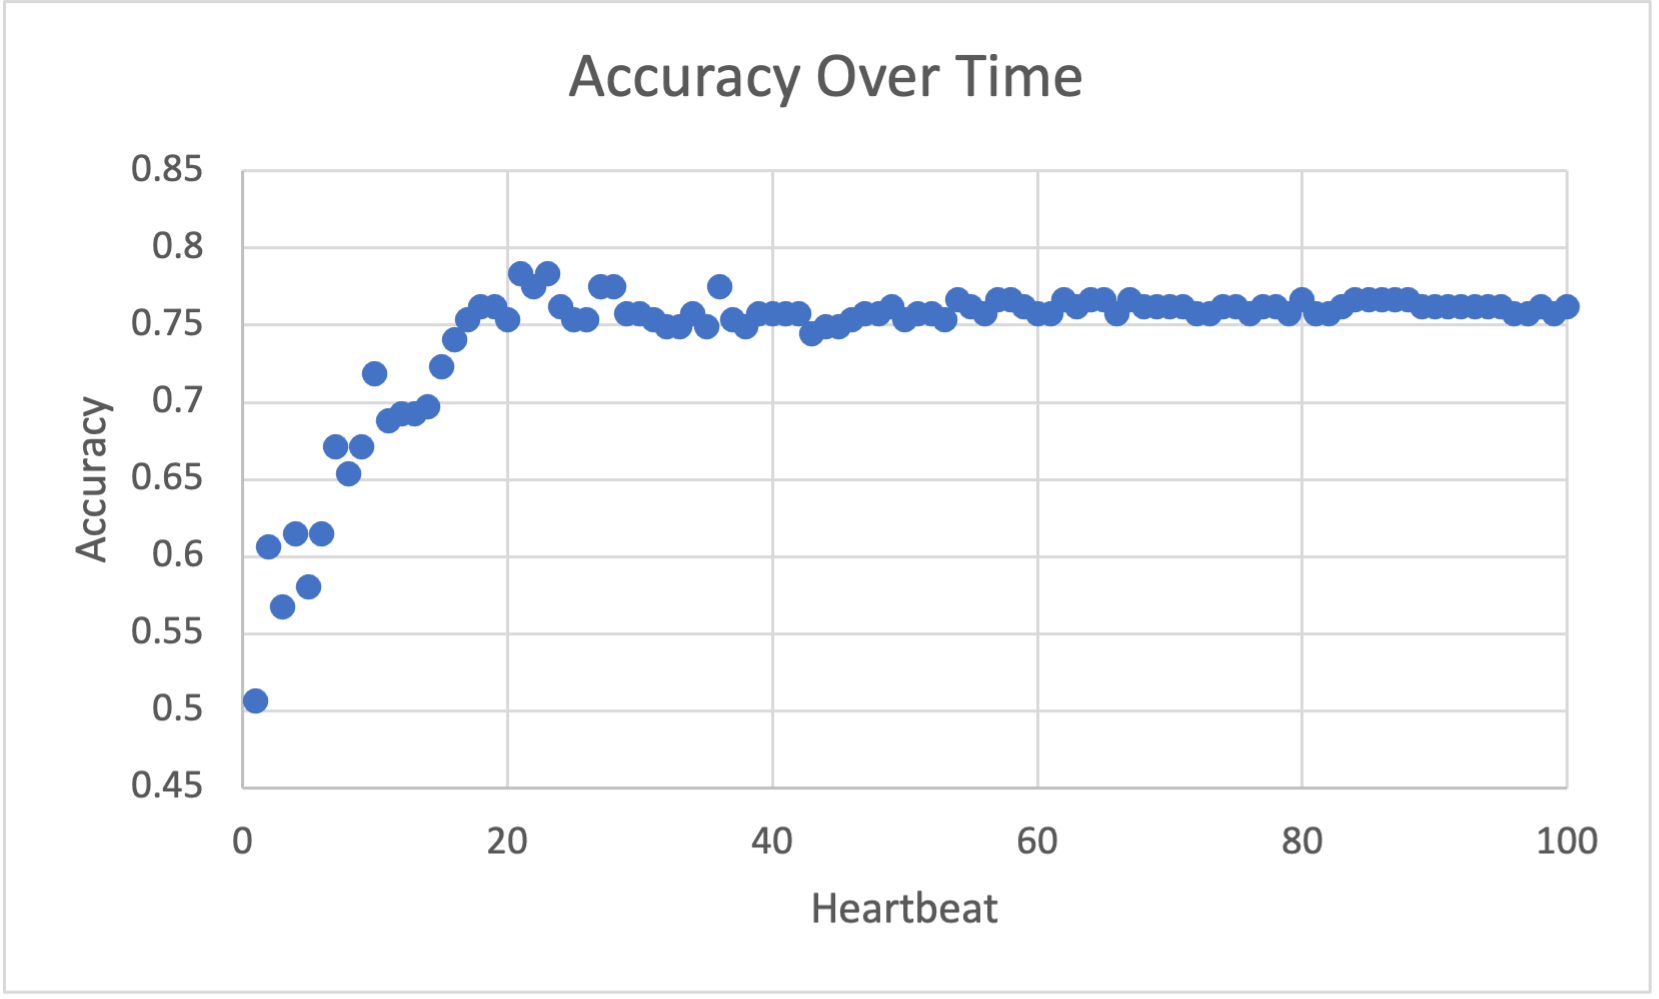
\includegraphics[width=0.5\textwidth]{accuracy.png}
    \caption{Accuracy of Model Over Time}
    \label{fig:accuracy}

\end{figure}

You can see in \nameref{fig:accuracy} that the model initially performs poorly (~50\% accuracy) after only being trained by the leader's data. However, overtime, as every node retrains the model multiple times with their data the model converges to ~75\% accuracy. As the number of heartbeats, and thus retrains, increases, the movement of the accuracy becomes less volatile. This is because each time the model is retrained it weights the addition based on the proportion of data it has already been trained on. 
\\
\\
The model's accuracy after distributed training is slightly worse than when trained in one pass on 70\% of the data set. This is likely because while the individual nodes continuously retrain the model, the leader does not. The leader only trains the model using its data one time. Thus overtime, the model is trained less and less on the leader's data. This is a limitation of our simulation, but not our distributed system. In order to resolve this issue, we would have actual users only update the model one time with every new set of data they acquire. In the real world, nodes may periodically acquire new data that they want to add to the network. Because our data set was limited in size and we focused on the distributed system, we did not implement the necessary UI for this.

\subsubsection{Technical Details}
We implemented the distributed system using gRPC as our wire protocol. 

\section{Challenges and Future Directions}

\subsection{Challenges, Learnings \& Limitations}
\label{sec:cll}
One issue we repeatedly ran in to while building our system was maintaining state variables between the gRPC server and the main function of a node or leader. For example, we wanted the gRPC server and main function to share the same set of active nodes, ML model, and heartbeat timer. In order to do this, we initialized objects in the main function and passed references of them to the gRPC server when we initialized it. You can see these objects in $node.py$, $model\_train.py$, $model.py$, $heartbeat\_timer.py$, and $active\_nodes.py$.

\\

Another issue we ran into involved our use of threads. We used threads to run the gRPC server and the main server for each node and the leader. This worked well, except when the leader received a deregistration call from a node and had to remove it from the set of active nodes. In a prior implementation of the code we held the set of active nodes in a list. When a node sent a deregister request, the leader would pop that node from the list. This caused the leader to crash as the size of the active node list decreased while a thread was looping through it. To solve this issue we used a dictionary to hold the set of active nodes. If a node deregistered then the value for that node would be set to None in the dictionary and wouldn't be sent a heartbeat or sent to the nodes in the active nodes list. This allowed us to remove the node from the active node list without causing the leader to crash.

\\

A limitation of our system is that at any moment when two or more nodes are up, they could each decide to send an updated model to the leader. Because the leader will not immediately send the updated model to the nodes, it is true that the node that sends the update second will override the update of the first node. Once the leader sends out the heartbeat the nodes will once again be synced. Because our distributed system involves only 5 nodes (that have a $\frac{1}{5}$ chance of updating the model), we did not run into this issue frequently and it did not have an effect on the performance of the model. However, if the system began to incorporate more nodes that updated the model more frequently, it would become an issue. One resolution would be for each node to send only changes in the weights of the model when trained on the new data and let the leader update the model itself. This would ensure the leader is able to incorporate both updates. Another resolution to this issue would be to have the leader send out a notification to all other nodes that they should wait to send updates until they receive the next heartbeat from the leader with the updated model. This would ensure that the leader is able to incorporate both updates however, it would introduce a worse user experience with more latency. 


\subsection{Future Directions}
There are a number of future directions that can be taken with this project. One direction would be to implement a UI for the system. This would allow users to choose which model they want to update as well as allow them to upload new data. Users would also be able to see the accuracy of the model over time. With a UI we would be able to implement security and verification of users such that certain models could only be seen or retrained by specific users. These features would be necessary for a real world implementation of this system.
\\
Another future direction of this project would be to implement a better way of handling concurrent updates to the same model by different nodes. As mentioned in \nameref{sec:cll}, this could be done by having the leader update the model itself or by having the leader notify the nodes to wait to send updates until they receive the next heartbeat. 
\\
Finally, one could implement a more complex system that retrains using a number of different algorithms. Individual nodes could then run inference on whichever model they wanted. This would allow for a more complex system that could be used for a variety of different applications. 

\end{document}